% Drawing 138/06-14 -- folder 138, batch 06, archive page 109 (PDF page 110).
% Transcription: à l'encre, un petit arbre inscrit dans une lentille, avec des arêtes vers l'extérieur. Au crayon, sur la moitié inférieure : une carte à faces hachurées, sommets marqués $2$, $4$, $8$, $2$, $4$, $8$, $2$, un segment pointillé ; des courbes emboîtées qui se referment vers un sommet marqué $8$ ; plus bas, un axe allant vers $\infty$ et une figure de cercles concentriques traversée par un segment.
% Kind: maps over a typed notice (ink tree in a lens; pencil maps, nested curves, circles). Method 2 (schematic redraw from the facsimile). Status: partial.
% Notes: Drawn over a typed departmental notice (a thesis-defence announcement naming the candidate and the jury; the typed text is left out of the redraw, but the contact-sheet crop shows it). Ink: a small tree inscribed in a lens, with two edges going out to marked points. Pencil, lower half: a map with hatched faces and vertices marked 2, 4, 8, 2, 4, 8, 2, a dotted segment; nested curves closing towards the vertex 8 at the right; below, an axis running to infinity at the left and a figure of concentric circles crossed by a segment, with short edges. The many long faint parallel strokes are not drawn, and the nested curves are approximate; the pencil « 2(Sigma p + Sigma q + Sigma r) = 6N » is text.
% Coordinates: 1 unit = 1 mm = 1/100 of the crop width (bbox in page fractions: [0.1, 0.5, 0.9, 0.9]).
% Redrawn by Claude (claude-opus-5-5), issue #73, 2026-11-07; not checked by a human; not compiled (no TeX in the session).
% Rights: reproduces part of the work -- behind RENDER_TRANSCRIPTS, never published by itself.
\documentclass[tikz,border=3pt]{standalone}
\usepackage{amsmath,amssymb}
\usetikzlibrary{patterns,arrows.meta}
\tikzset{pencil/.style={black!45}, struck/.style={black!35}, mark/.style={circle,draw,inner sep=1.3pt}, pt/.style={circle,fill,inner sep=0.9pt}, opt/.style={circle,draw,fill=white,inner sep=1.1pt}}
\begin{document}
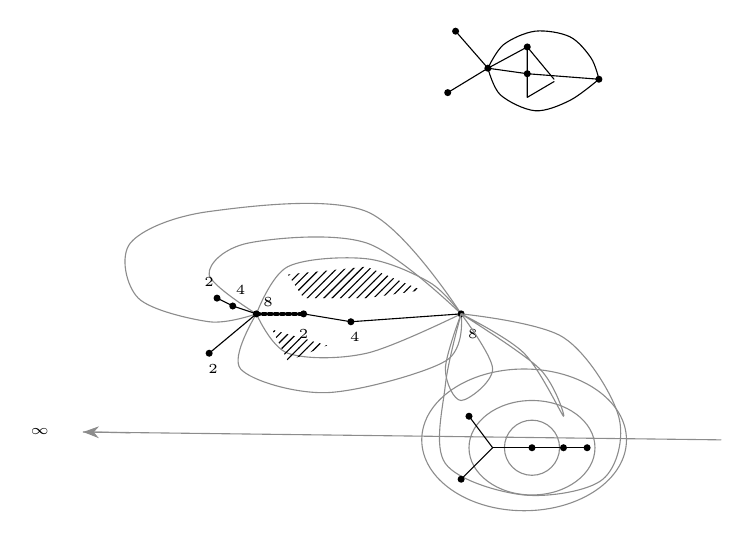
\begin{tikzpicture}[x=1mm,y=1mm,line cap=round,line join=round,font=\scriptsize]
\draw plot[smooth, tension=0.55] coordinates {(65.4,-8.6) (67.4,-5.6) (71.4,-3.9) (75.8,-4.6) (78.5,-7.3) (79.5,-10)};
\draw plot[smooth, tension=0.55] coordinates {(65.4,-8.6) (67,-12) (71.4,-14) (75.8,-12.7) (79.5,-10)};
\draw (65.4,-8.6) -- (70.4,-9.3) -- (79.5,-10);
\draw (70.4,-9.3) -- (70.4,-5.9) -- (73.8,-10);
\draw (70.4,-9.3) -- (70.4,-12.3) -- (73.8,-10.3);
\draw (65.4,-8.6) -- (70.4,-5.9);
\draw (65.4,-8.6) -- (61.3,-3.9);
\draw (65.4,-8.6) -- (60.3,-11.7);
\node[pt] at (65.4,-8.6) {};
\node[pt] at (70.4,-9.3) {};
\node[pt] at (70.4,-5.9) {};
\node[pt] at (79.5,-10) {};
\node[pt] at (61.3,-3.9) {};
\node[pt] at (60.3,-11.7) {};
\draw[pencil] plot[smooth, tension=0.55] coordinates {(62,-39.8) (50,-26.8) (30,-26.8) (20,-30.8) (21,-37.8) (30,-40.8) (36,-39.8)};
\draw[pencil] plot[smooth, tension=0.55] coordinates {(36,-39.8) (30,-34.8) (35,-30.8) (50,-30.8) (62,-39.8)};
\draw[pencil] plot[smooth, tension=0.55] coordinates {(36,-39.8) (40,-33.8) (50,-32.8) (58,-35.8) (62,-39.8)};
\draw[pencil] plot[smooth, tension=0.55] coordinates {(36,-39.8) (40,-44.8) (50,-44.8) (62,-39.8)};
\draw[pencil] plot[smooth, tension=0.55] coordinates {(36,-39.8) (34,-46.8) (45,-49.8) (60,-45.8) (62,-39.8)};
\fill[pattern=north east lines] (40,-34.8) -- (50,-33.8) -- (57,-36.8) -- (50,-37.8) -- (42,-37.8) -- cycle;
\fill[pattern=north east lines] (38,-41.8) -- (45,-43.8) -- (40,-45.8) -- cycle;
\draw[densely dotted,very thick] (36,-39.8) -- (42,-39.8);
\draw (42,-39.8) -- (48,-40.8) -- (62,-39.8);
\draw (36,-39.8) -- (33,-38.8) -- (31,-37.8);
\draw (36,-39.8) -- (30,-44.8);
\node[pt] at (31,-37.8) {};
\node[pt] at (33,-38.8) {};
\node[pt] at (36,-39.8) {};
\node[pt] at (42,-39.8) {};
\node[pt] at (48,-40.8) {};
\node[pt] at (62,-39.8) {};
\node[pt] at (30,-44.8) {};
\node[inner sep=1pt] at (30,-35.8) {\tiny $2$};
\node[inner sep=1pt] at (34,-36.8) {\tiny $4$};
\node[inner sep=1pt] at (37.5,-38.3) {\tiny $8$};
\node[inner sep=1pt] at (42,-42.3) {\tiny $2$};
\node[inner sep=1pt] at (48.5,-42.8) {\tiny $4$};
\node[inner sep=1pt] at (63.5,-42.3) {\tiny $8$};
\node[inner sep=1pt] at (30.5,-46.8) {\tiny $2$};
\draw[pencil] plot[smooth, tension=0.55] coordinates {(62,-39.8) (66,-46.8) (62,-50.8) (60,-46.8) (62,-39.8)};
\draw[pencil] plot[smooth, tension=0.55] coordinates {(62,-39.8) (70,-44.8) (75,-52.8) (72,-46.8) (62,-39.8)};
\draw[pencil] plot[smooth, tension=0.55] coordinates {(62,-39.8) (75,-42.8) (82,-52.8) (80,-60.8) (70,-62.8) (60,-58.8) (60,-48.8) (62,-39.8)};
\draw[pencil] (14,-54.8) -- (95,-55.8);
\draw[-{Stealth[length=2mm]},pencil] (20,-54.9) -- (14,-54.8);
\node[inner sep=1pt] at (8.5,-54.8) {\tiny $\infty$};
\draw[pencil] (71,-56.8) circle[radius=3.5];
\draw[pencil] (71,-56.8) ellipse[x radius=8, y radius=6];
\draw[pencil] (70,-55.8) ellipse[x radius=13, y radius=9];
\draw (66,-56.8) -- (78,-56.8);
\draw (66,-56.8) -- (63,-52.8);
\draw (66,-56.8) -- (62,-60.8);
\node[pt] at (71,-56.8) {};
\node[pt] at (75,-56.8) {};
\node[pt] at (78,-56.8) {};
\node[pt] at (63,-52.8) {};
\node[pt] at (62,-60.8) {};
\end{tikzpicture}
\end{document}
